\documentclass[a4paper,12pt]{article}

\usepackage[T2A]{fontenc}			
\usepackage[utf8]{inputenc}			
\usepackage[english,russian]{babel}	

\usepackage[
bookmarks=true, colorlinks=true, unicode=true,
urlcolor=black,linkcolor=black, anchorcolor=black,
citecolor=black, menucolor=black, filecolor=black,
]{hyperref}

\usepackage{color}
\usepackage{caption}
\DeclareCaptionFont{white}{\color{black}}
\DeclareCaptionFormat{listing}{\colorbox{white}{\parbox{\textwidth}{#1#2#3}}}
\captionsetup[lstlisting]{format=listing,labelfont=white,textfont=white}

\usepackage{amsmath,amsfonts,amssymb,amsthm,mathtools} 
\usepackage{wasysym}

\usepackage[cache=false]{minted}

\usepackage{graphicx}
%\usepackage[cache=false]{minted}
\usepackage{cmap}
\usepackage{indentfirst}

\usepackage{listings} 
\usepackage{fancyvrb}

\usepackage{geometry}
\geometry{left=2cm}
\geometry{right=1.5cm}
\geometry{top=1cm}
\geometry{bottom=2cm}

\setlength{\parindent}{5ex}
\setlength{\parskip}{0.5em}

\usepackage{pgfplots}

\usepackage{longtable}

\begin{document}
	\lstset{ %
		language=C,                 % выбор языка для подсветки (здесь это С)
		basicstyle=\small\sffamily, % размер и начертание шрифта для подсветки кода
		numbers=left,               % где поставить нумерацию строк (слева\справа)
		numberstyle=\tiny,           % размер шрифта для номеров строк
		stepnumber=1,                   % размер шага между двумя номерами строк
		numbersep=5pt,                % как далеко отстоят номера строк от подсвечиваемого кода
		backgroundcolor=\color{white}, % цвет фона подсветки - используем \usepackage{color}
		showspaces=false,            % показывать или нет пробелы специальными отступами
		showstringspaces=false,      % показывать или нет пробелы в строках
		showtabs=false,             % показывать или нет табуляцию в строках
		frame=single,              % рисовать рамку вокруг кода
		tabsize=2,                 % размер табуляции по умолчанию равен 2 пробелам
		captionpos=t,              % позиция заголовка вверху [t] или внизу [b] 
		breaklines=true,           % автоматически переносить строки (да\нет)
		breakatwhitespace=false, % переносить строки только если есть пробел
		escapeinside={\%*}{*)}   % если нужно добавить комментарии в коде
	}
	
	% Титульный лист
	\begin{figure}[h!]
		\begin{center}
			{
\includegraphics[scale = 0.4]{img/titul.jpg}}
			\label{titul}
		\end{center}
	\end{figure}
	
	\vspace*{15mm} 
	
	\huge
	\begin{center}
		Дисциплина: <<Компьютерные сети>>
	\end{center}
	
	\begin{center}
		Лабораторная работа №8
	\end{center}

	
	\huge
	\begin{center}
		Тема работы:\\
		<<Изучение протоколов динамической маршрутизации RIPv2 и OSPF в сетевом симуляторе>>
	\end{center}
	\vspace*{25mm} 
	
	\large
	\begin{flushright}
		Студент: Левушкин И. К. \\
		Группа: ИУ7-72Б \\
		Преподаватель: Рогозин Н.О. \\
	\end{flushright}
	
	\vspace*{25mm}
	\begin{center}
		Москва, 2020 г.  
	\end{center}
	\thispagestyle{empty}
	
	
	\newpage
	
	\section{Назначить адреса подсетей}
	
	Подсети в соответствии вариантом $x = 7$:
	
	\begin{enumerate}
		\item Подсеть 1: 192.168.7.0/24
		\item Подсеть 2: 192.168.8.0/24
		\item Подсеть 3: 192.168.9.0/24
		\item Подсеть 4: 192.168.10.0/24
		\item Подсеть 5 (в задаче 3): 192.168.17.0/24
	\end{enumerate}

	Подсети стенда I обозначены на рисунке 1. Адреса выданы с помощью
протокола DHCP (как в лр 6, 7). Роутерам стенда I адреса выданы статически.
Пример выдачи адреса для хоста подсети 1 представлен на рисунке 2.

Стенд II настраивается аналогично. В 5 подсети роутер 7 выступает в качестве DHCP-сервера.

	\begin{figure}[h!]
		\begin{center}
			{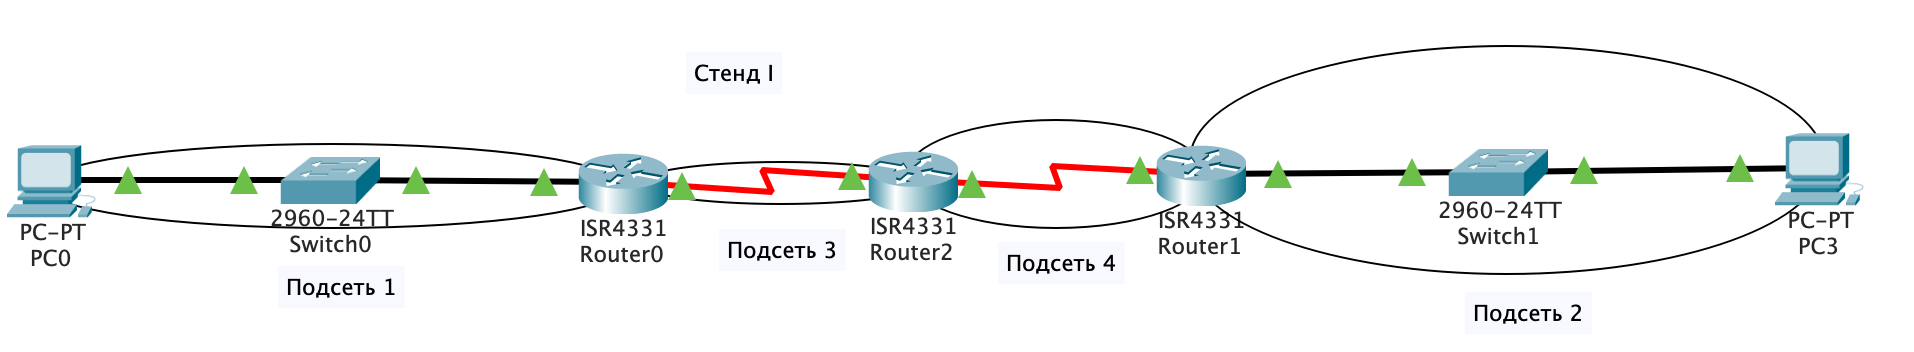
\includegraphics[width = \textwidth]{img/1.png}}
			\caption{}
			\label{ris:1}
		\end{center}
	\end{figure}

	\newpage

	\begin{figure}[h!]
		\begin{center}
			{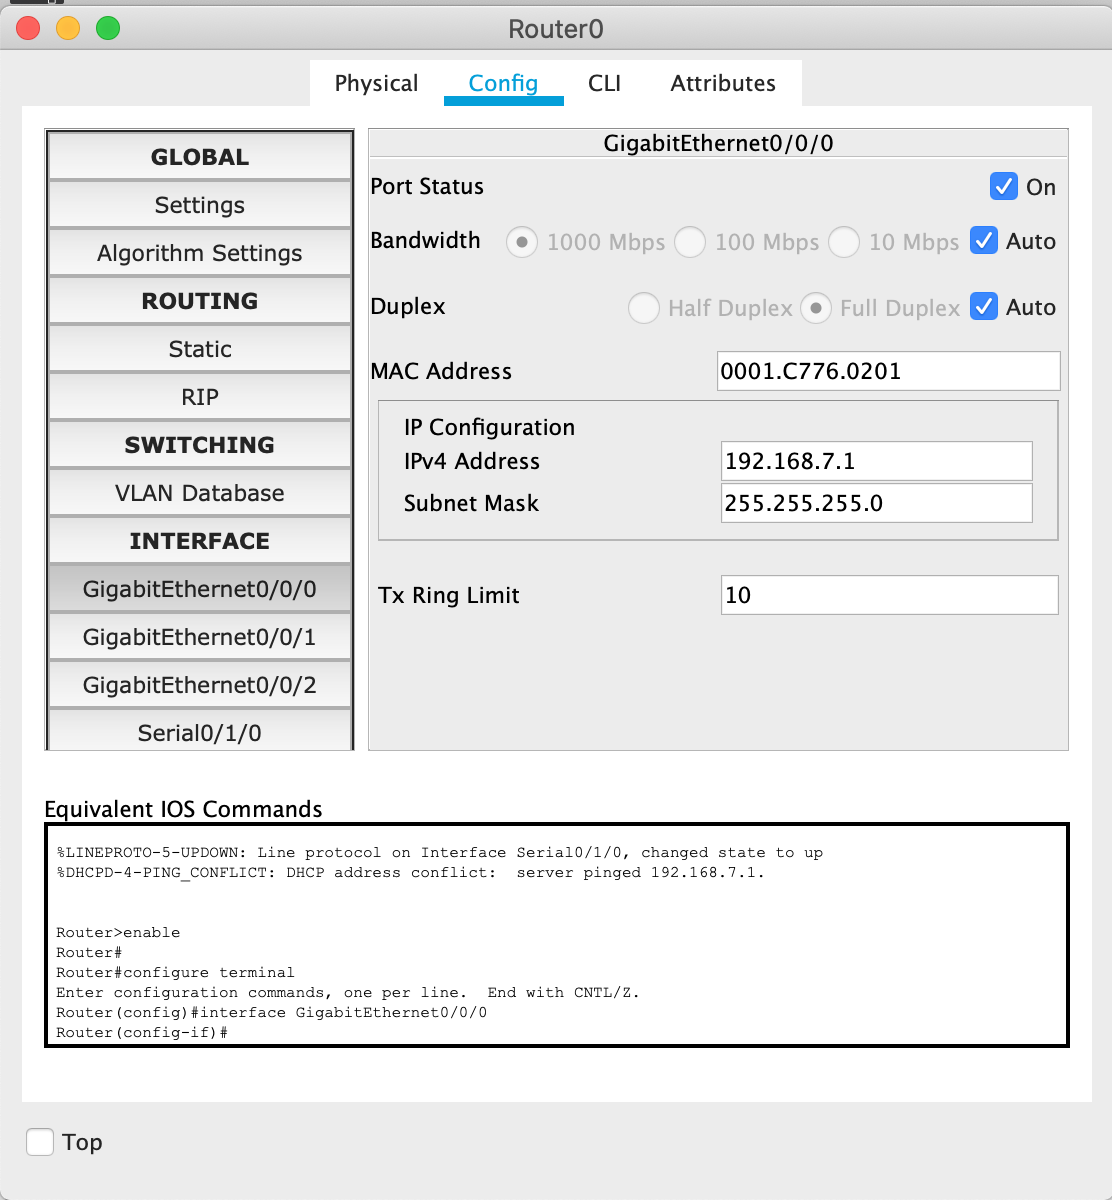
\includegraphics[scale = 0.45]{img/2.png}}
			\caption{}
			\label{ris:2}
		\end{center}
	\end{figure}

	\begin{figure}[h!]
		\begin{center}
			{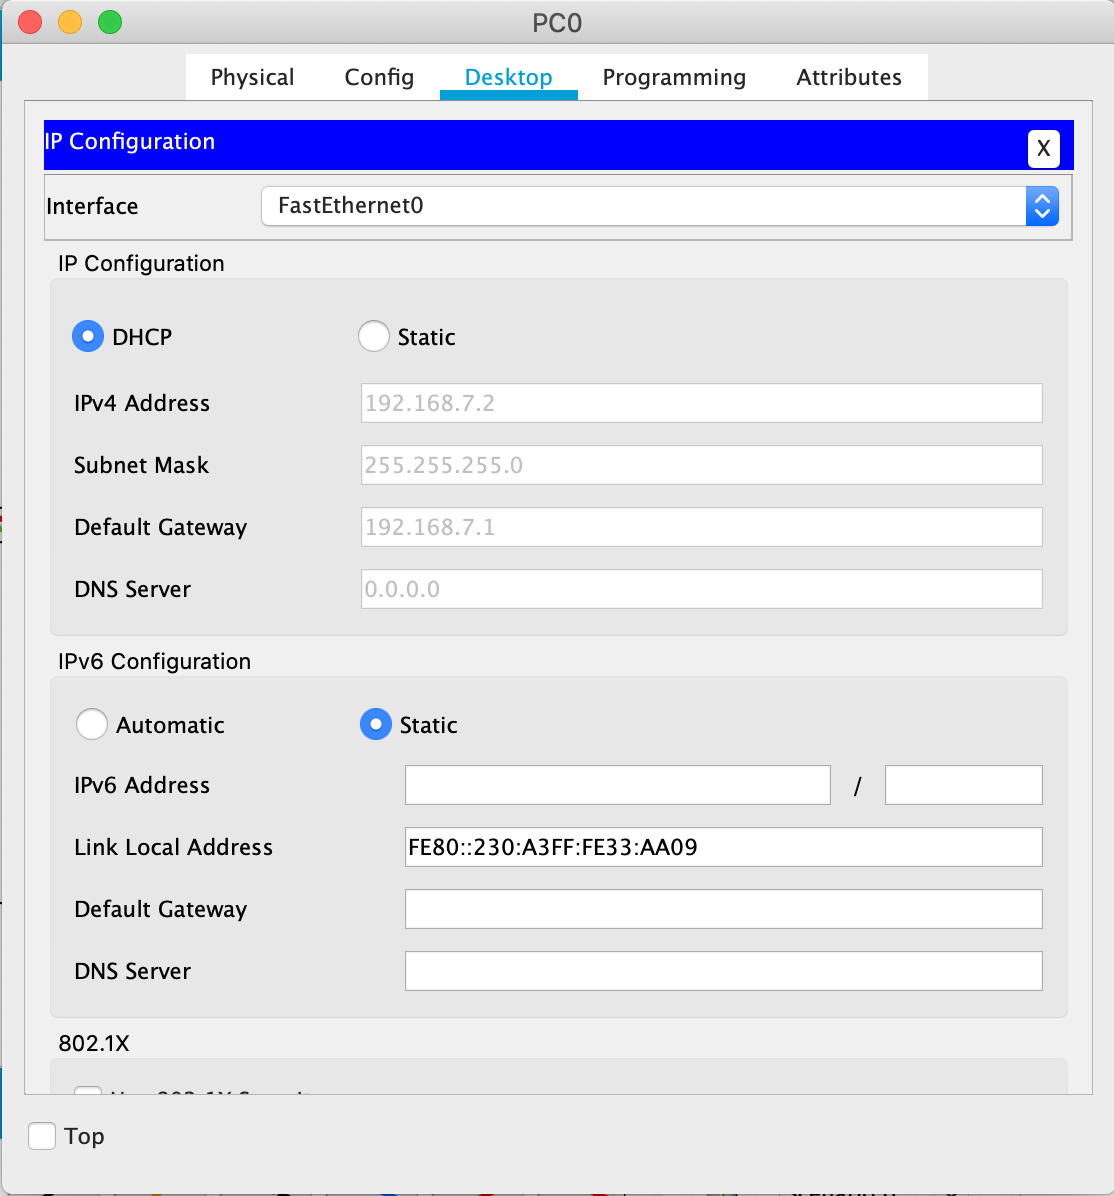
\includegraphics[scale = 0.45]{img/3.png}}
			\caption{}
			\label{ris:3}
		\end{center}
	\end{figure}

	\newpage

	\section{Настроить динамическую маршрутизацию в прилагаемом .pkt файле на стенде I через протокол RIPv2 так, чтобы пинг любым хостом или маршрутизатором любого другого хоста или маршрутизатора был успешным.}
	
	Роутер 0:
	
	\begin{itemize}
		\item router rip
		\item version 2
		\item network 192.168.7.0
		\item network 192.168.9.0
	\end{itemize}

Роутер 2:

\begin{itemize}
	\item router rip
	\item version 2
	\item network 192.168.9.0
	\item network 192.168.10.0
\end{itemize}

Роутер 1:

\begin{itemize}
	\item router rip
	\item version 2
	\item network 192.168.10.0
	\item network 192.168.8.0
\end{itemize}

\newpage

	\begin{figure}[h!]
		\begin{center}
			{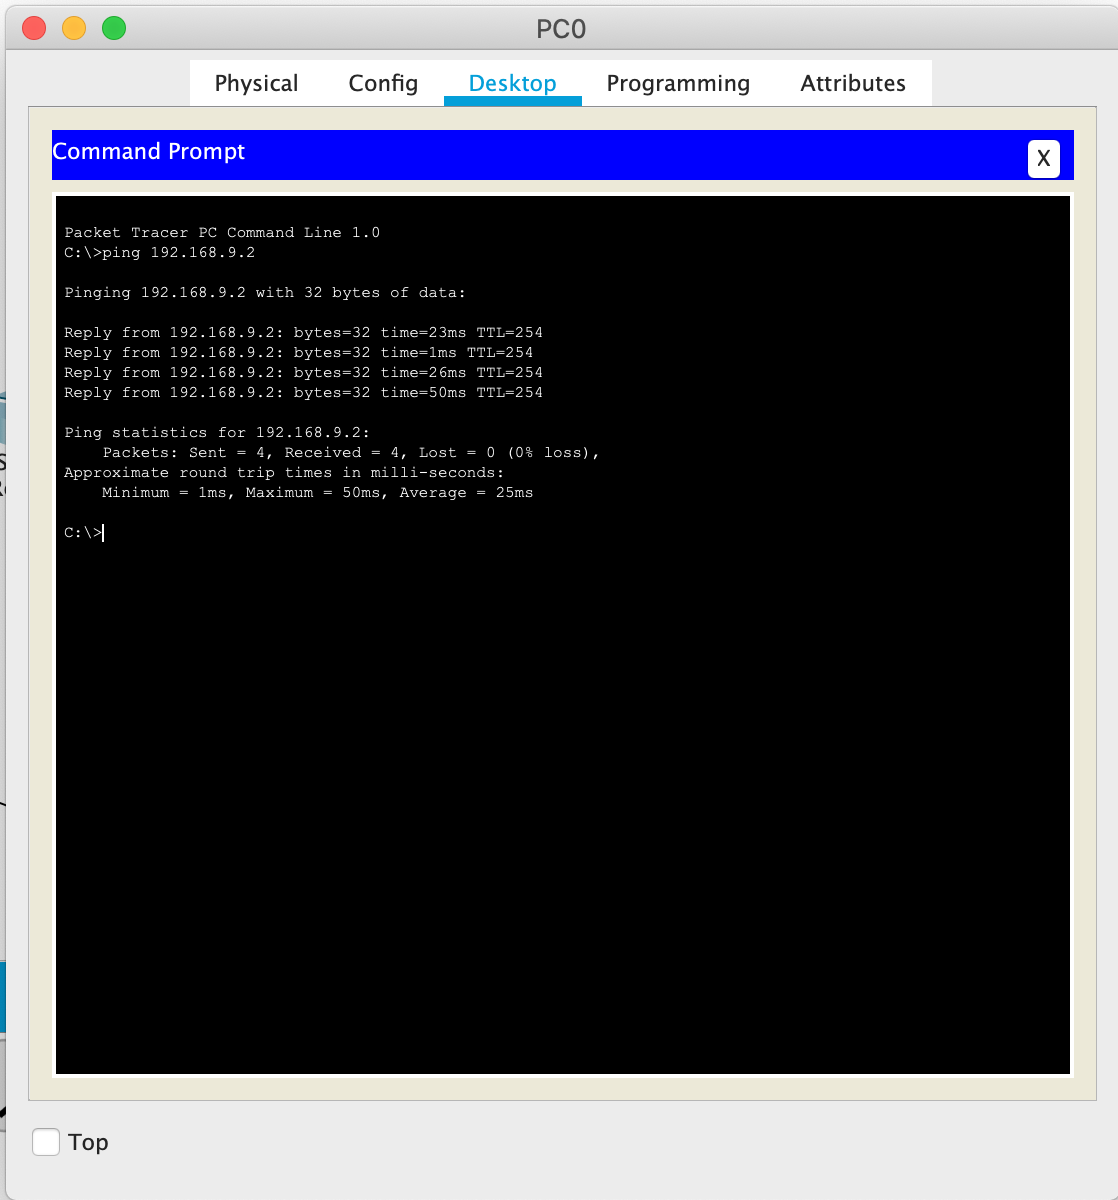
\includegraphics[scale = 0.45]{img/4.png}}
			\caption{}
			\label{ris:4}
		\end{center}
	\end{figure}

	\section{Настроить динамическую маршрутизацию в сети в прилагаемом .pkt файле на стенде II через протокол OSPF так, чтобы пинг любым хостом или маршрутизатором любого другого хоста или маршрутизатора был успешным. Разделить при этом сеть на области OSPF в соответствии со схемой. Выполнить указания в лабораторной работе.}
	
	Роутер 7:
	
	\begin{itemize}
		\item router ospf 1
		\item network 192.168.7.0 0.0.0.255 area 1
		\item network 192.168.17.0 0.0.0.255 area 0
		\item router-id 1.1.1.1
	\end{itemize}

	Роутер 8:
	
	\begin{itemize}
		\item router ospf 1
		\item network 192.168.8.0 0.0.0.255 area 2
		\item network 192.168.17.0 0.0.0.255 area 0
		\item router-id 2.2.2.2
	\end{itemize}

	Роутер 9:
	
	\begin{itemize}
		\item router ospf 1
		\item network 192.168.9.0 0.0.0.255 area 3
		\item network 192.168.17.0 0.0.0.255 area 0
		\item router-id 3.3.3.3
	\end{itemize}

	Роутер 10:
	
	\begin{itemize}
		\item router ospf 1
		\item network 192.168.10.0 0.0.0.255 area 4
		\item network 192.168.17.0 0.0.0.255 area 0
		\item router-id 4.4.4.4
	\end{itemize}

	\begin{figure}[h!]
		\begin{center}
			{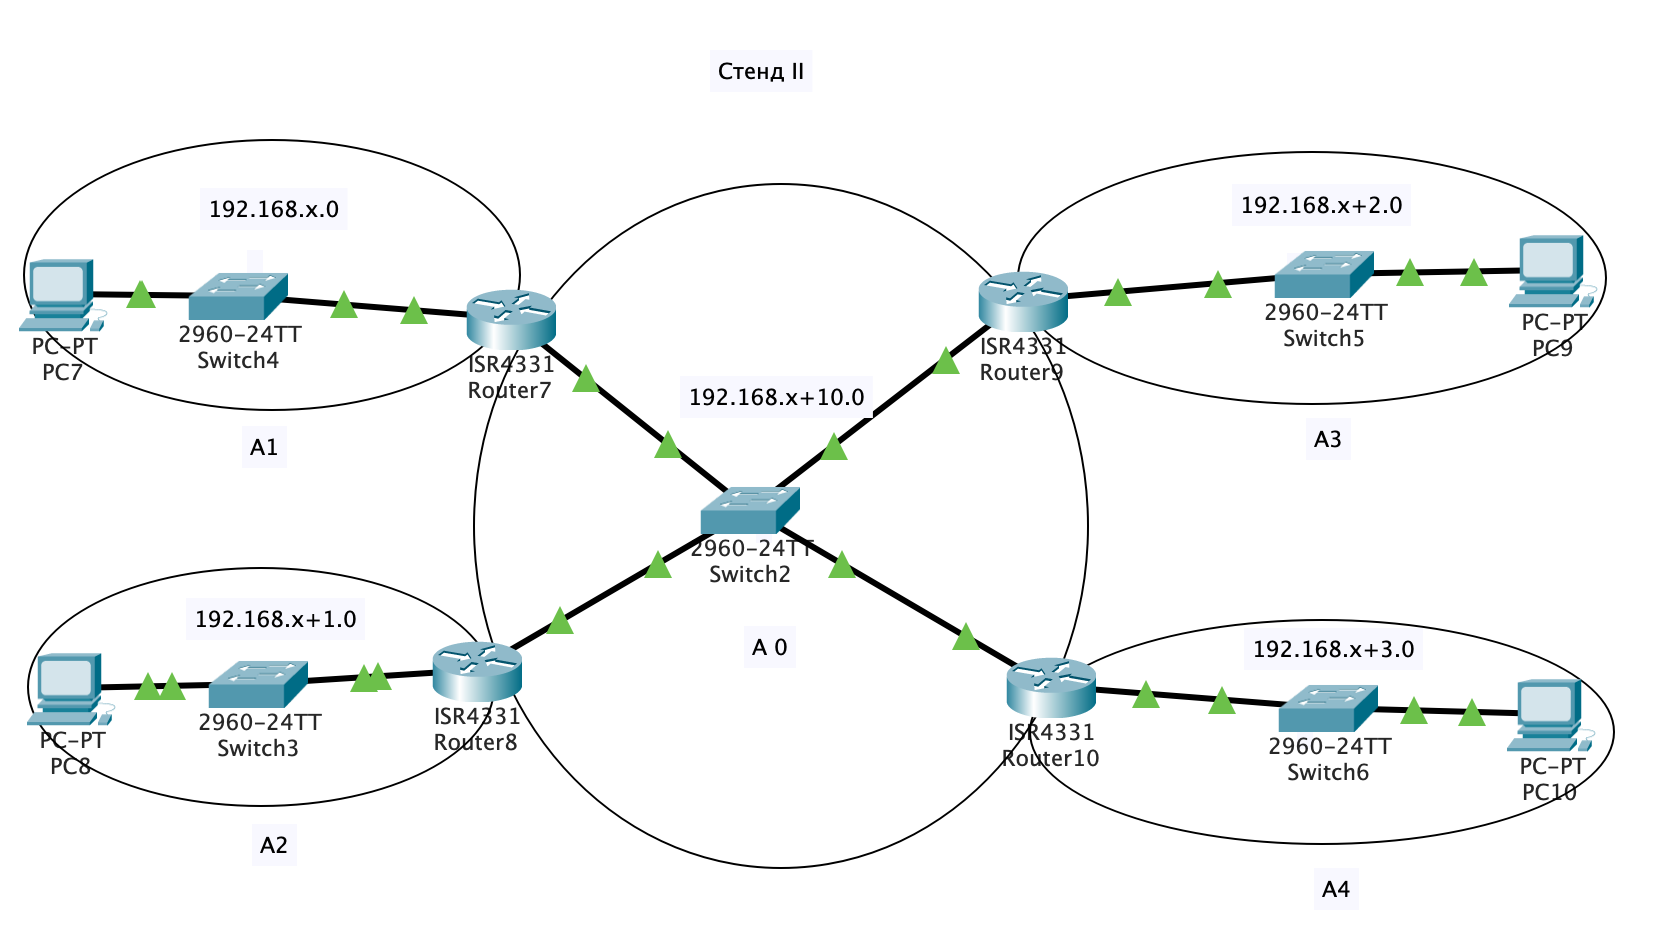
\includegraphics[width = \textwidth]{img/5.png}}
			\caption{}
			\label{ris:5}
		\end{center}
	\end{figure}

	\newpage

	\begin{figure}[h!]
		\begin{center}
			{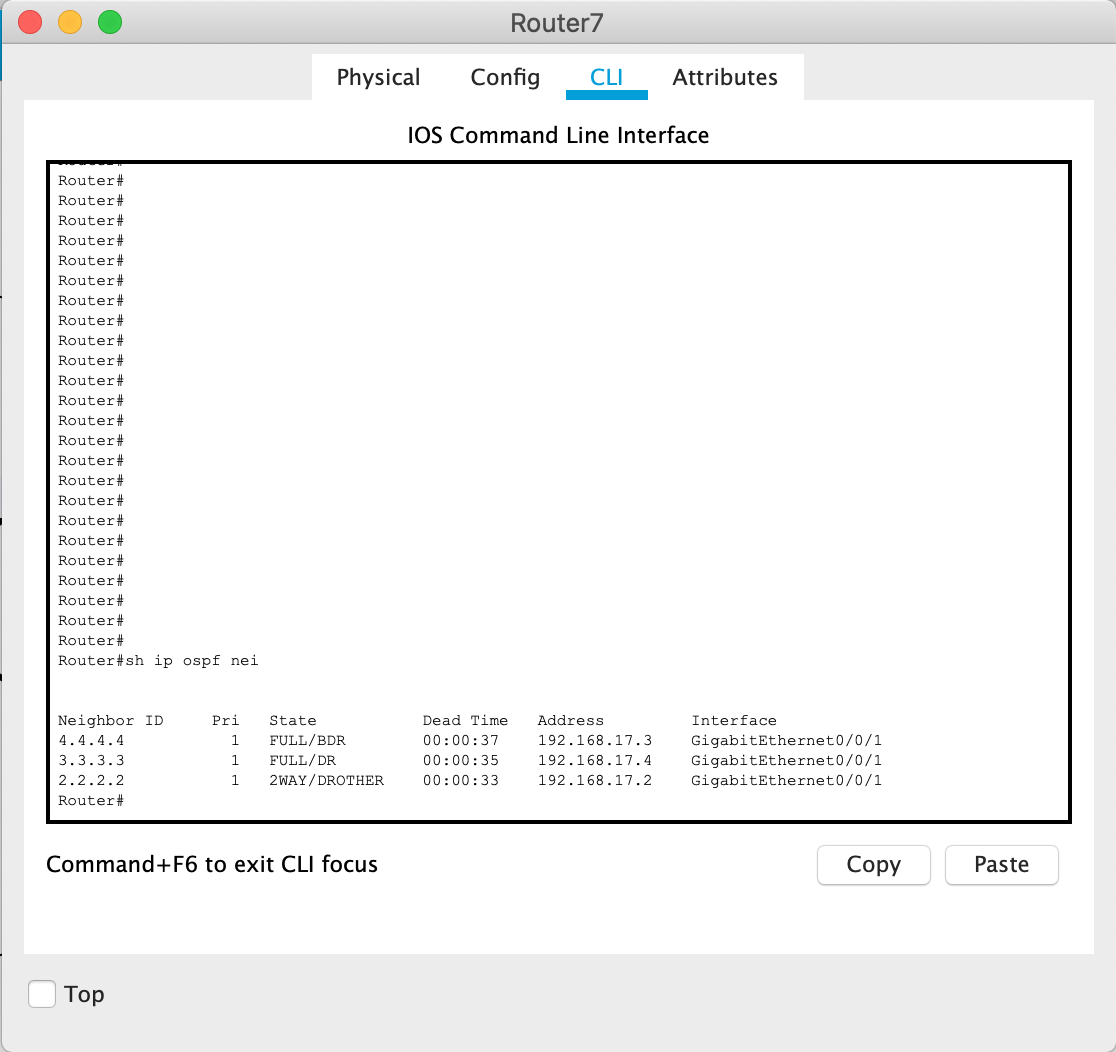
\includegraphics[scale = 0.6]{img/6.png}}
			\caption{}
			\label{ris:6}
		\end{center}
	\end{figure}

	Аутентификация на роутере 7 для подсети A1:
	
	\begin{itemize}
		\item int gigabitEthernet 0/0/0
		\item ip ospf authentication-key 4321
		\item exit
		\item router ospf 1
		\item area 1 authentication
	\end{itemize}

	\begin{figure}[h!]
		\begin{center}
			{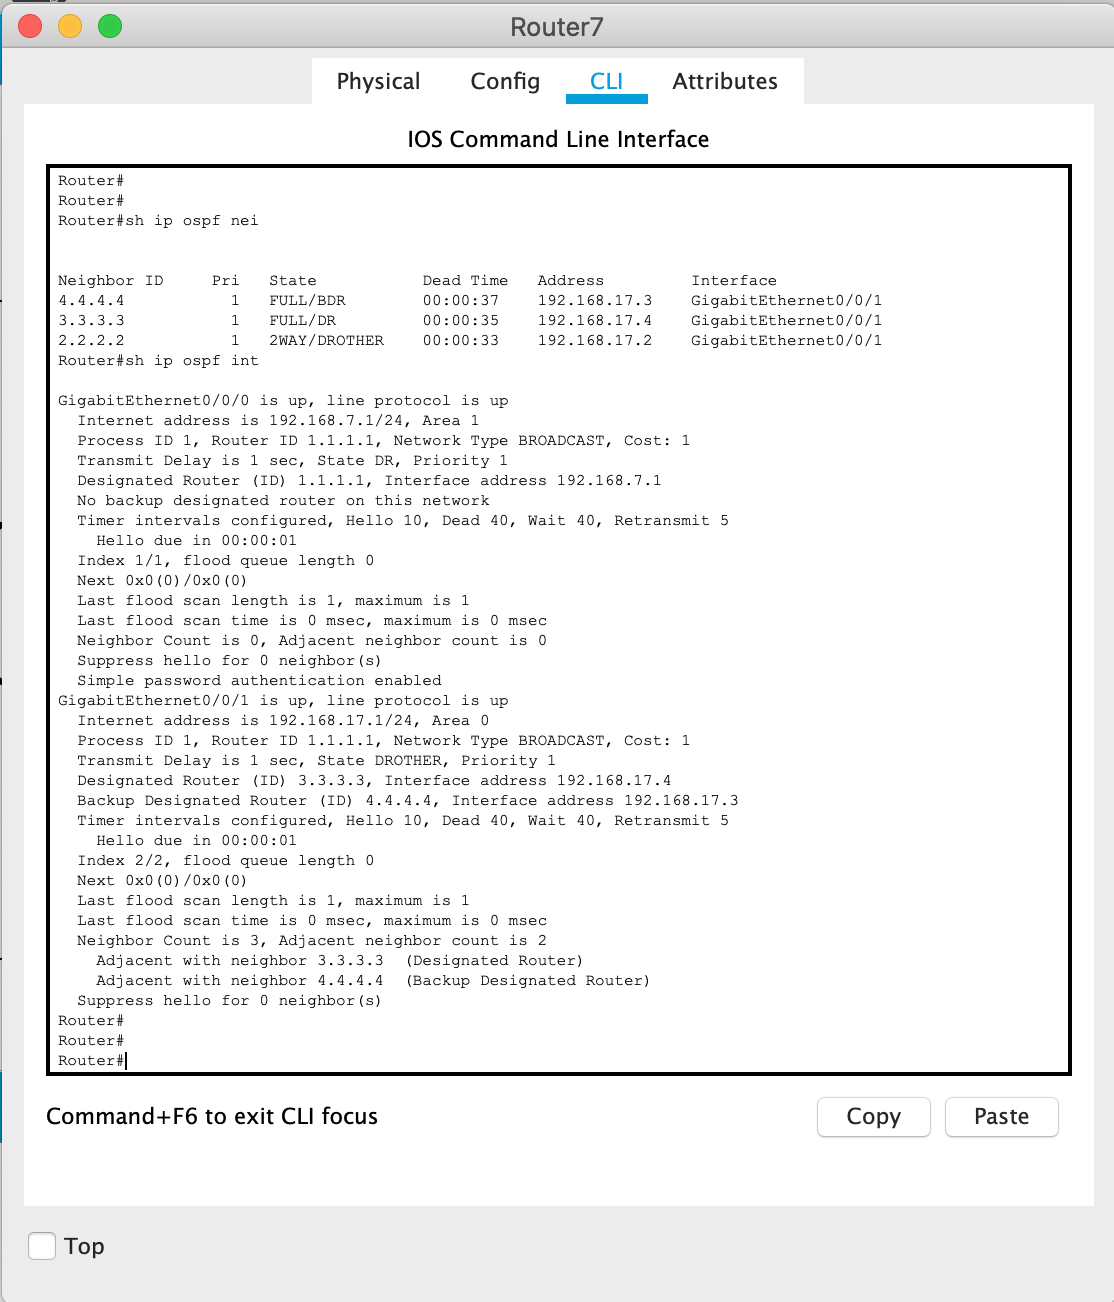
\includegraphics[width = \textwidth]{img/7.png}}
			\caption{}
			\label{ris:7}
		\end{center}
	\end{figure}
	
\end{document}